\documentclass{standalone}
\usepackage{tikz}
\begin{document}

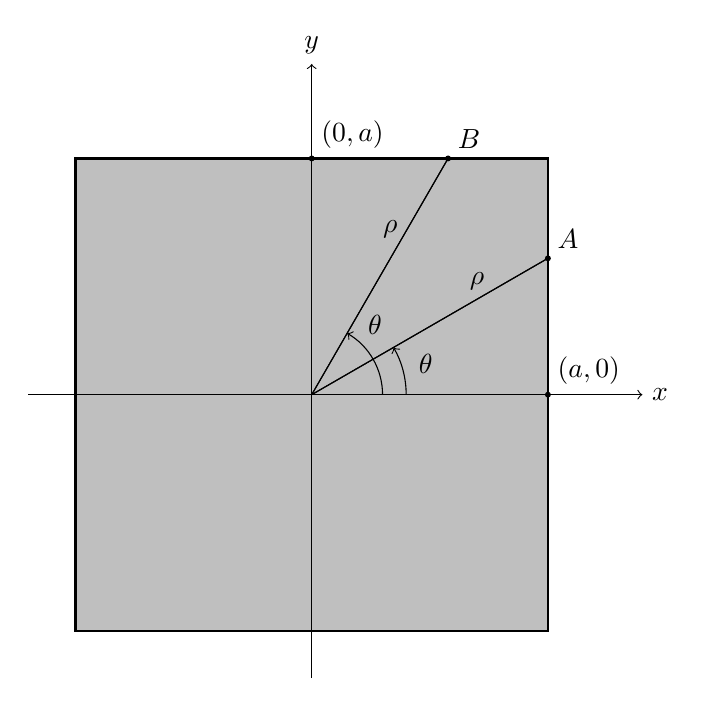
\begin{tikzpicture}[scale=3]

  % square
  \filldraw[fill=lightgray, thick] (1,-1) -- (1,1) -- (-1,1) -- (-1,-1) -- cycle;

  % Draw axes
  \draw[->] (-1.2,0) -- (1.4,0) node[right] {$x$};
  \draw[->] (0,-1.2) -- (0,1.4) node[above] {$y$};

  \def\eps{0.01}
  \filldraw (1,0) circle (\eps) node[anchor=south west] {$(a,0)$};
  \filldraw (0,1) circle (\eps) node[anchor=south west] {$(0,a)$};

  \def\thetaval{30}
  % Compute the endpoint: (1, tan 35�)
  \path (1,{tan(\thetaval)}) coordinate (P);
  % Draw line from origin to intersection
  \draw[] (0,0) -- (P);
  % Mark the point
  \filldraw (P) circle (\eps) node[above right] {$A$};
  \draw[->] (0.4,0) arc[start angle=0, end angle=\thetaval, radius=0.4];
  \node at (\thetaval/2:0.5) {$\theta$};
  \draw (0,0) -- (P) node[pos=0.7, above] {$\rho$};

  \def\thetaval{60}
  % Compute the endpoint: (1, tan 35�)
  \path ({1/tan(\thetaval)}, 1) coordinate (P);
  % Draw line from origin to intersection
  \draw[] (0,0) -- (P);
  % Mark the point
  \filldraw (P) circle (\eps) node[above right] {$B$};
  \draw[->] (0.3,0) arc[start angle=0, end angle=\thetaval, radius=0.3];
  \node at (0.8*\thetaval:0.4) {$\theta$};
  \draw (0,0) -- (P) node[pos=0.7, anchor=east] {$\rho$};

  %=================================================
  % Polar coordinates
  \def\theta{40} % angle in degrees
  \def\r{1}      % radius

  % Point in polar coordinates
  % \coordinate (P) at (\theta:\r);

  % Draw radius vector
  % \draw[->, thick, blue] (0,0) -- (P) node[midway, above right] {$r$};

  % Draw angle arc
  % \draw[->, red] (0.4,0) arc[start angle=0, end angle=\theta, radius=0.4];
  % \node at (0.55,0.15) {$\theta$};

  % Mark the point
  % \filldraw[red] (P) circle (0.03) node[above right] {$(r,\theta)$};

\end{tikzpicture}

\end{document}
